%!TEX root = ../main.tex
% file: problem2.tex
\section{Stirling Numbers} % (fold)
\label{sec:stirling_numbers}
We wish to generate Stirling numbers of the first kind which are calculated using the recurrence
\begin{equation}
    \label{eq:stirling}
    c(n,k) = -(n-1)\times c(n-1,k) + c(n-1,k-1), \mbox{for } n \ge1 \mbox{ and } k \ge 1
\end{equation}
and the initial conditions $c(n,k)=0$ if $n\le0$ or $k\le0$, and $c(0,0)=1$. We intend to write a script which contains a class with the recursive function as well a dictionary which may be used to store previous values.

\subsection{Program Description} % (fold)
\label{sub:program_description2}
We begin by creating a class who's initializer contains a dictionary for previously stored values.
\begin{lstlisting}[caption={Initialization}, label=lst:init2,firstnumber=3]
    def __init__(self, n, k):
        self.dict = {(0,0):1} #start with the initial condition (saves an if statement)
        self.answer = self.c(n,k)
\end{lstlisting}\noindent
In Listing \ref{lst:init2} we populate the dictionary \emph{self.dict} with one of our initial conditions: $c(0,0)=1$. This is done to avoid an additional conditional statement in the main routine.
\begin{lstlisting}[caption={Main Logic for Stirling Number Generation}, label=lst:main2,firstnumber=8]
    def c(self, n, k):
         """Computes stirling numbers either recursively or by looking up in dictionary"""
         if (n,k) in self.dict.keys():
             return self.dict[(n,k)]
         elif n<=0 or k<=0:
             return 0
         else:
             ans = - (n-1)*self.c(n-1,k) + self.c(n-1,k-1)
             self.dict[(n,k)] = ans
             return ans
\end{lstlisting}\noindent
In \ref{lst:main2} we see that there is a conditional statement with three possible conditions. We first check if the solution is already available in our dictionary to prevent unnecessary recursion and calculation; the second check performed is whether we are at an initial condition $n\le0$ or $k\le0$. Finally, if it is not an initial condition and we do not have the value in our dictionary, we calculate the result of Eq. \ref{eq:stirling}.
% subsection program_description (end)

\subsection{Results} % (fold)
\label{sub:results2}
A quick test was initially performed on the code to see whether it was producing the correct result. We called the class with the values $n=5$ and $k=2$ with the following results:
\begin{figure}[H]
    \centering
        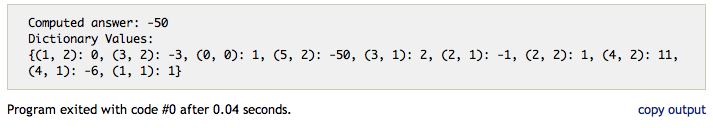
\includegraphics[width=6in]{include/prob2test.png}
    \caption{Testing of Program 2}
    \label{fig:include_prob2test}
\end{figure}
In Fig. \ref{fig:include_prob2test} we see the result $c(5,2)=-50$ which is the signed result. There was no specification of whether to produce signed or unsigned Stirling numbers, therefore they were left as signed. Similarly the dictionary is seen to have all necessary Stirling numbers from the recursion.



% subsection results (end)
% section stirling_numbers (end)